\section{Returns modeling}
\label{sec:randomness_assets}
Return is defined as the percentage growth in the value of an asset, together with accumulated dividends, over some period \citep{pw_iqf2ed_2007}:
\begin{equation}
    \text{Return} = \frac{\text{change in value of the asset + accumulated cash flows}}{\text{original value of the asset}}
\end{equation}

Denoting the asset value on the $i$-th day by $S_i$ then the return from day $i$ to day $i+1$ is given by:
\begin{equation}
     R_i = \frac{S_{i+1} - S_i}{S_i}
\end{equation}
The dividends are ignored here, they are easily allowed for, especially since they only get
paid two or four times a year typically. 

The mean of the returns distribution is:
\begin{equation}
    \text{mean} = \bar{R} = \frac{1}{M} \sum_{i = 1}^{M} R_i
    \label{equ:mean}
\end{equation}
and the sample standard deviation is:
\begin{equation}
    \text{sd} = \sqrt{\frac{1}{M-1} \sum_{i = 1}^{M} \left( R_i - \bar{R} \right)^2}
    \label{equ:std}
\end{equation}
where $M$ is the number of returns in the sample (one fewer than the number of asset prices). 

Figures \ref{fig:daily_return}(a,b) show the quoted price of a stock and its daily return in the duration considered. The daily return looks very much like `noise' and is modeled as such. Corresponding to the data in the example, the mean is 0.002916 and the standard deviation is 0.024521. Notice how the mean daily return is much smaller than the standard deviation. This is very typical of financial quantities over short timescales. On a day-by-day basis you will tend to see the noise in the stock price, and will have to wait months perhaps before you can spot the trend.

The frequency distribution of this time series of daily returns is plotted in Figure \ref{fig:daily_return}(c), it has been scaled and translated to give it a mean zero, a standard deviation of one and an area under the curve of one. This distribution is fairly close to the standardized normal distribution of
\begin{equation}
    \frac{1}{\sqrt{2\pi}} e^{-\frac{1}{2}\phi^2}
\end{equation}
where $\phi$ is a standardized normal variable.

Then, it is possible to assume that the returns can be modeled as a random variable drawn from a normal distribution with a know, constant, non-zero mean and a known, constant, non-zero standard deviation:
\begin{equation}
    R_i = \frac{S_{i+1} - S_i}{S_i} = \text{mean} + \text{sd} \times \phi
\end{equation}

\begin{figure}[H]
    \centering
    \begin{subfigure}[b]{0.3\textwidth}
        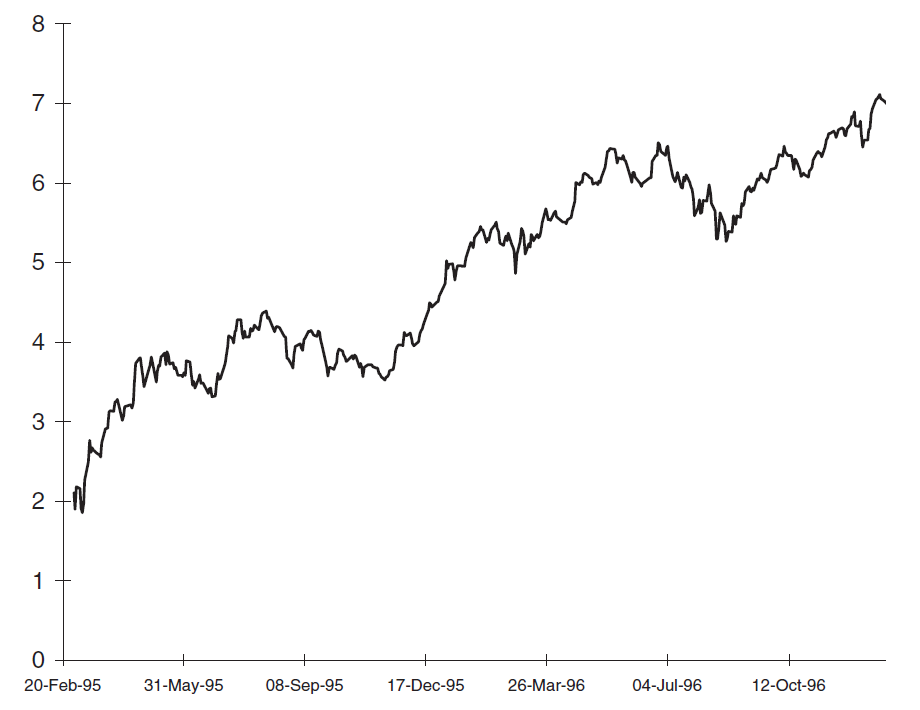
\includegraphics[width=\textwidth]{figure/daily_return_1.png}
        \caption{Quoted price of a stock}
    \end{subfigure}
    \begin{subfigure}[b]{0.3\textwidth}
        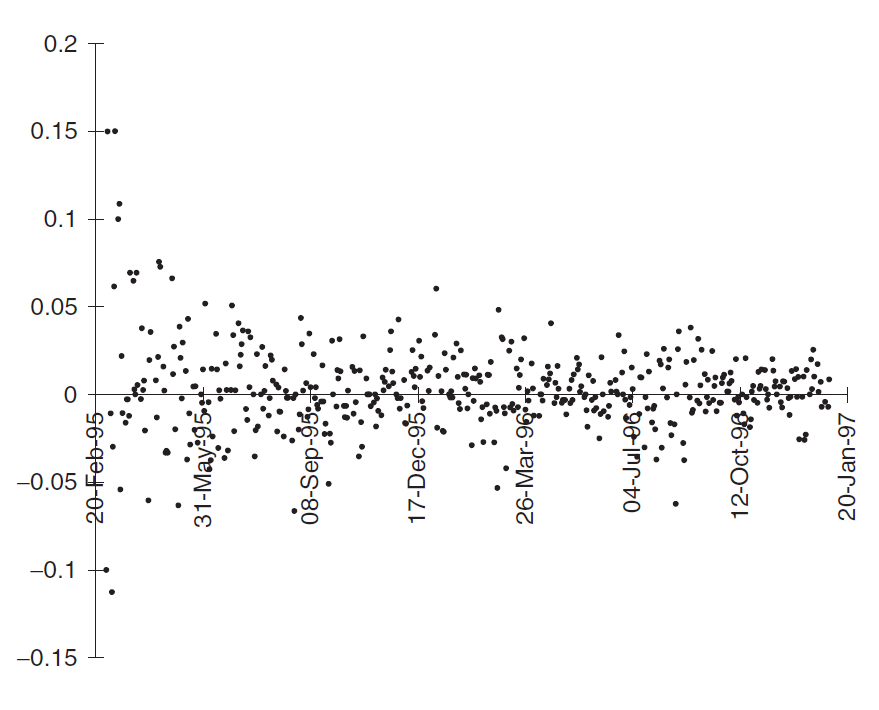
\includegraphics[width=\textwidth]{figure/daily_return_2.png}
        \caption{Daily returns}
    \end{subfigure}
    \begin{subfigure}[b]{0.3\textwidth}
        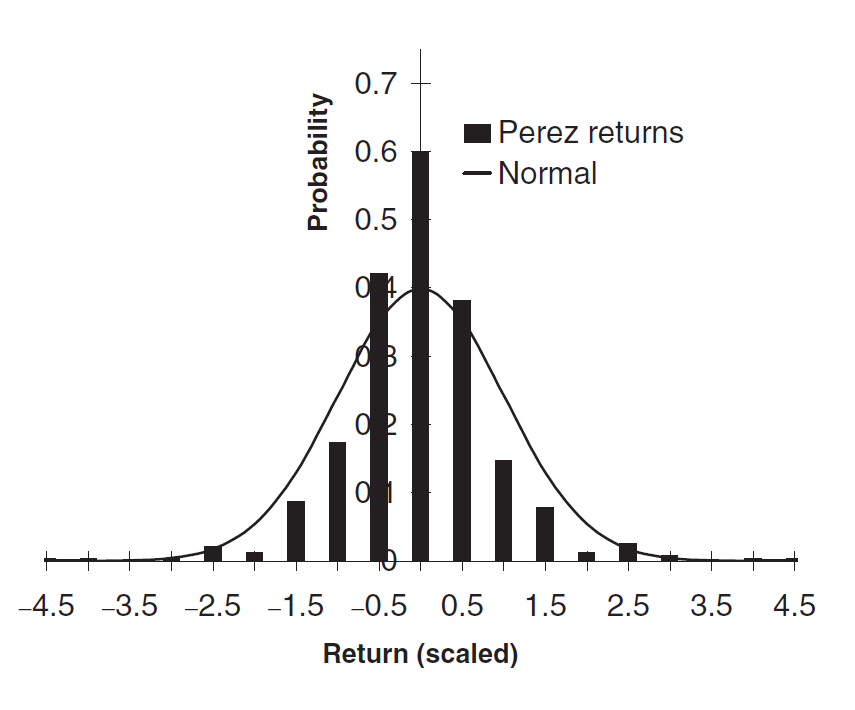
\includegraphics[width=\textwidth]{figure/daily_return_3.png}
        \caption{Norm. frequency distribution}
    \end{subfigure}
    \caption{Example of a daily return}
    \label{fig:daily_return}
\end{figure}



\subsection{Discrete-time model}
In reality, the assets may be measured in different time scale, i.e. hourly, daily, weekly... hence we need to take into account the time step in modeling returns. Call the time step $\delta t$. Following Equation \ref{equ:mean}, it is reasonable to assume that the return scales with the size of the time step as follows:
\begin{equation}
    \text{mean} = \mu \; \delta t
\end{equation}
for some $\mu$ which is assumed to be constant now. Similarly, following Equation \ref{equ:std}, the standard deviation of the asset return over a time step $\delta t$ must be $O \left( \delta t^{1/2} \right)$:
\begin{equation}
    \text{sd} = \sigma \; \delta t^{1/2}
\end{equation}
where $\sigma$ is some parameter measuring the amount of randomness, the larger this parameter the more uncertain is the return. And the asset return model becomes:
\begin{equation}
    R_i = \frac{S_{i+1} - S_i}{S_i} = \mu \; \delta t + \sigma \; \phi \; \delta t^{1/2}
\end{equation}
or:
\begin{equation}
    S_{i+1} - S_i = \mu \; S_i \; \delta t + \sigma \; S_i \; \phi \; \delta t^{1/2} 
\end{equation}   
The left-hand side of this equation is the change in the asset price from time step $i$ to time step $i+1$. The right-hand side is the `model'. We can think of this equation as a model for a \textbf{random walk}\index{random walk} of the asset price.

The parameter $\mu$ is called the \textbf{drift rate}\index{drift rate}, the \textbf{expected return}\index{expected return} or the \textbf{growth rate}\index{growth rate} of the asset. It can be estimated by:
\begin{equation}
    \mu = \frac{1}{M \delta t} \sum_{i = 1}^{M} R_i
    \label{equ:drift}
\end{equation}
Statistically it is very hard to measure since the mean scales with the usually small parameter $\delta t$. The unit of time that is usually used is the year, in which case $\mu$ is quoted as an annualized growth rate. In the classical option pricing theory the drift plays almost no role. So even though it is hard to measure, this doesn't matter too much \cite{pw_iqf2ed_2007}.

The parameter $\sigma$ is called the \textbf{volatility}\index{volatility} of the asset. It can be estimated by:
\begin{equation}
    \sigma = \sqrt{\frac{1}{\left( M - 1 \right) \delta t} \sum_{i = 1}^{M} \left( R_i - \bar{R} \right)^2}
    \label{equ:volatility_1}
\end{equation}
Again, this is almost always quoted in annualized terms. The volatility is the most important and elusive quantity in the theory of derivatives. If $\delta t$ is sufficiently small, the mean return $\bar{R}$ term can be ignored; and in this case, the following equation:
\begin{equation}
    \sigma = \sqrt{\frac{1}{\left( M - 1 \right) \delta t} \sum_{i = 1}^{M} \left( \log S(t_i) - \log S(t_{i-1}) \right)^2}
    \label{equ:volatility_2}
\end{equation}
can be used where $S(t_i)$ is the closing price on day $t_i$.

Because of their scaling with time, the drift and volatility have different effects on the asset path. The drift is not apparent over short timescales for which the volatility dominates. Over long timescales, for instance decades, the drift becomes important.

It is highly unlikely that volatility is constant for any given asset. Changing economic circumstances, seasonality, etc. will inevitably result in volatility changing with time. If
you want to know the volatility today you must use some past data in the calculation.  Unfortunately, this means that there is no guarantee that you are actually calculating today's volatility. Typically you would use daily closing prices to work out daily returns and then use the past 10, 30, 100, ... daily returns in the formula above.

\begin{figure}[H]
    \centering
    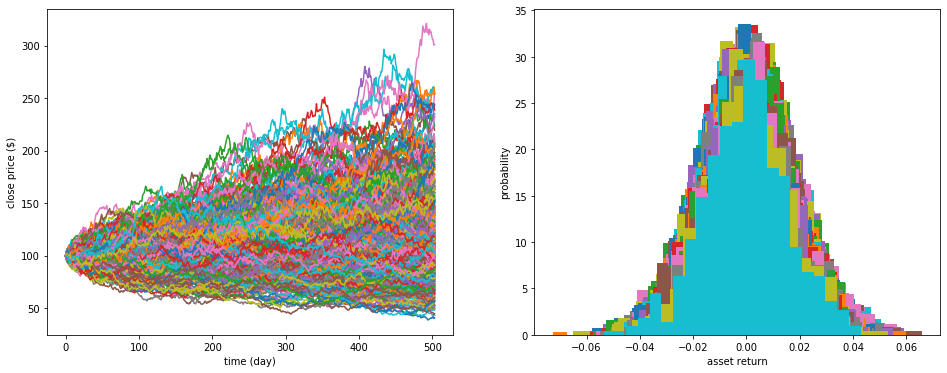
\includegraphics[width=\textwidth]{figure/random walk.png}
    \caption{Random walk model for an asset and corresponding return}
    \label{fig:random_walk_500}
\end{figure}

Figure \ref{fig:random_walk_500} reproduces the random walk model presented in Section 4.8 \cite{pw_iqf2ed_2007} for 500 evolution scenarios of an asset with the initial value of \$100, the drift rate $\mu$ of 0.10, the volatility $\sigma$ of 0.25, a daily quote in two-year duration. The corresponding asset returns of those 500 scenarios are also calculated, it can be seen that the asset returns closely follow the normal distribution as expected. Python code for this basic model can be found \href{https://github.com/chitn/quantfin_study/blob/master/code/asset_modeling-random_walk.py}{here}.



\subsection{Continuous-time model}
The random walk model described in the previous section has a discrete time step; in this section, a brief introduction to the continuous-time limit of the random walk model is presented as a starting point for the world of stochastic modeling and Wiener processes. These topics will be presented in more detailed in Section \ref{sec:stochastic_calculus}.

We rewrite the asset return model here for convenience:
\begin{equation}
    S_{i+1} - S_i = \mu \; S_i \; \delta t + \sigma \; S_i \; \phi \; \delta t^{1/2}
\end{equation}

First we introduce a quantity $dS$ representing \textit{the change in} the asset price in \textit{continuous time}, i.e. we go to the limit $\delta t = 0$. So the left-hand side becomes $dS$. The first $\delta t$ in the right-hand side can also translate into $dt$. 

For the second term of the right-hand side, however, we can not straightforwardly translate $\delta t^{1/2}$ into $dt^{1/2}$ \textit{otherwise any random $dt^{1/2}$ will dominate any deterministic $dt$ term}. It turns out, we will see in Section \ref{sec:stochastic_calculus}, that because the variance of the random term is $O(\delta t)$ we can make a sensible continuous-time limit of our discrete-time model. The term $\phi \delta t^{1/2}$ is rewritten as $dX$ which can be thought as a random variable drawn from a normal distribution with mean zero and variance $dt$, i.e. $E[dX] = 0$ and $E[dX^2] = dt$. This is called a Wiener process. It should be noted that \textit{this is not exactly what it is but it is close enough}, the important point is that we can build up a continuous-time theory using Wiener processes instead of normal distribution and discrete time. 

The asset price model in the continuous-time limit using the Wiener process notation can be written as:
\begin{equation}
    dS = \mu \; S \; dt + \sigma \; S \; dX
\end{equation}
This is our first stochastic differential equation. It is a continuous-time model of an asset price. It is the most widely accepted model for equities, currencies, commodities and indices, and the foundation of so much finance theory. This equation will be derived following different approaches in next sections.


